\subsection{Building a mesh}

\begin{frame}
    \frametitle{Examples}

    \begin{figure}[!ht]
        \centering
        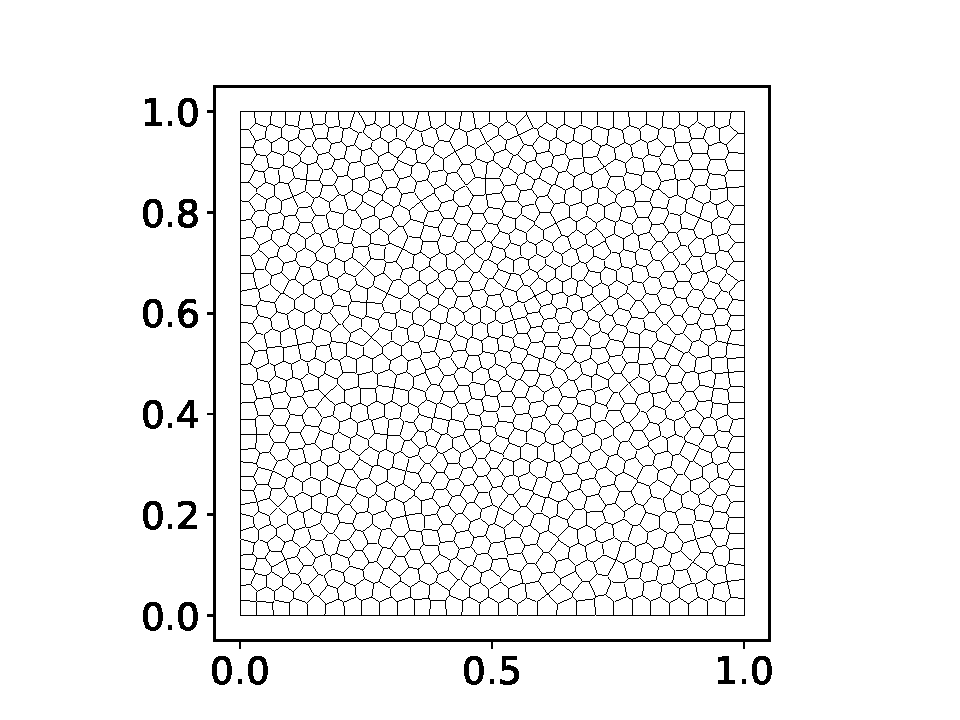
\includegraphics[trim=2cm 0.5cm 2cm 0.5cm, clip, width=0.45\textwidth]{meshes/uniform/square_1000.pdf}
        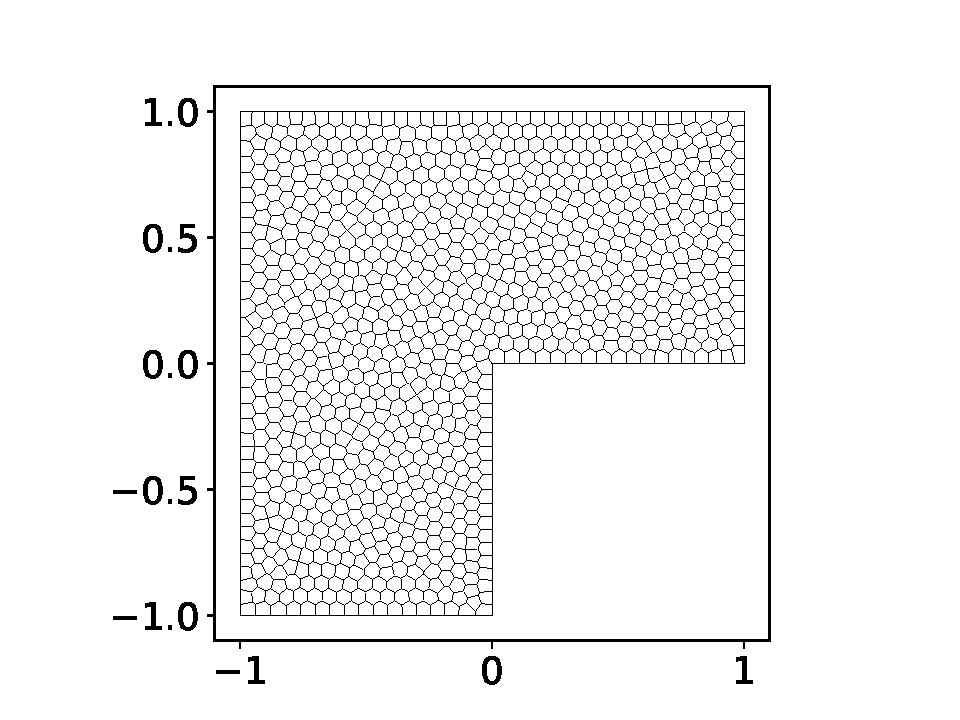
\includegraphics[trim=2cm 0.5cm 2cm 0.5cm, clip, width=0.45\textwidth]{meshes/uniform/lshape_1000.pdf}
        \caption{Square and L-shaped meshes over polygonal domains with $N = 1000$ elements.}
    \end{figure}
\end{frame}

\begin{frame}
    \frametitle{Mesh-building strategy}

    The mesh-building strategy involves the following steps:

    \begin{enumerate}
        \item Generate a Voronoi diagram to partition the domain into regions based on point locations.
        \item Refine the mesh by adjusting point positions to minimize element distortion.
        \item Remove or adjust very small edges to enhance mesh quality and stability.
        \item Analyze the connectivity and arrangement of mesh elements to ensure proper structure.
        \item Calculate properties such as element areas and the largest simplices.
    \end{enumerate}

    This is made possible through a comprehensive implementation of the necessary analytic geometry, such as operations between lines and polygons.

\end{frame}

\begin{frame}[fragile]
    \frametitle{\lstinline{mesh_diagram}, \lstinline{mesh_relax}}

    Most steps of the mesh-building process are carried out by \lstinline{mesh_diagram}\footnote{Building and postprocessing.} and \lstinline{mesh_relax}.

    \begin{lstlisting}[style=cpp]
    std::vector<Polygon> mesh_diagram(
        const Polygon &, 
        const std::size_t &, 
        const bool &reflect = false, 
        const bool &uniform = false);

    std::vector<Polygon> mesh_relax(
        const Polygon &, 
        const std::vector<Polygon> &, 
        const bool &reflect = false);
    \end{lstlisting}

\end{frame}

\begin{frame}[fragile]
    \frametitle{\lstinline{Mesh}}

    \lstinline{struct Mesh} requires a polygonal domain, a diagram, and information on the elements' degrees.

    \begin{lstlisting}[style=cpp]
    Mesh(
        const Polygon &, 
        const std::vector<Polygon> &, 
        const std::vector<std::size_t> &);

    Mesh(
        const Polygon &, 
        const std::vector<Polygon> &, 
        const std::size_t &degree = 1);
    \end{lstlisting}

\end{frame}

\begin{frame}[fragile]
    \frametitle{\lstinline{Mesh} methods}

    The following methods are invoked by the mesh constructors to evaluate the diagram's properties.

    \begin{lstlisting}[style=cpp]
    std::vector<Element> mesh_elements(
        const std::vector<Polygon> &, 
        const std::vector<std::size_t> &);

    std::vector<std::vector<std::array<int, 3>>> 
    mesh_neighbours(
        const Polygon &, 
        const std::vector<Element> &);

    std::vector<Real> mesh_areas(
        const std::vector<Polygon> &);

    std::vector<Vector<Real>> mesh_max_simplices(
        const std::vector<Polygon> &);
    \end{lstlisting}

\end{frame}

\subsection{Code examples}

\begin{frame}[fragile]
    \frametitle{A code snippet}

    The steps to create a mesh are schematized as follows:

    \begin{lstlisting}[style=cpp]
    Point a{0.0, 0.0};
    Point b{1.0, 0.0};
    Point c{1.0, 1.0};
    Point d{0.0, 1.0};

    Polygon domain{{a, b, c, d}};

    std::vector<Polygon> diagram = 
        mesh_diagram(domain, 100);
    
    Mesh mesh{domain, diagram};
    \end{lstlisting}

\end{frame}

\begin{frame}[fragile]
    \frametitle{Using the repository}

    Building a mesh over a square or L-shaped domain is as simple as calling one of the two scripts provided with the repository.

    To create a mesh over a square domain with $N = 250$, simply compile the domain scripts by:

    \begin{lstlisting}
    make domains
    \end{lstlisting}

    and then use the \lstinline{square_domain} script by:

    \begin{lstlisting}
    ./executables/square_domain.out 250
    \end{lstlisting}

\end{frame}